\documentclass{beamer}
\usepackage{listings}
\usetheme{Copenhagen}
\usecolortheme{beaver}
\setbeamertemplate{navigation symbols}{}
\setbeamertemplate{footline}{\parbox[t][12pt][c]{12pt}{~\scriptsize\insertframenumber}}
% \usepackage{beamerthemesplit} // Activate for custom appearance

\title{Declarative Cartography}
\subtitle{In-Database Map Generalization of Spatial Datasets}
\author{Pimin Konstantin Kefaloukos, Marcos Vaz Salles, Martin Zachariasen}
\date{\today}

\begin{document}

\frame{\titlepage}

% MOTIVATION
\frame
{
  \frametitle{Motivation}
  \begin{itemize}
  \item Zoomable map based on vector data (new data daily)
  \item At lower scales: too many objects to fit the map
  \item Map should balance \emph{representation} and  \emph{legibility}~\footnote{This map of tourism POI has only representation, not legibility}
  \item We need \emph{generalization} that is easy!
  \end{itemize}

  \fbox{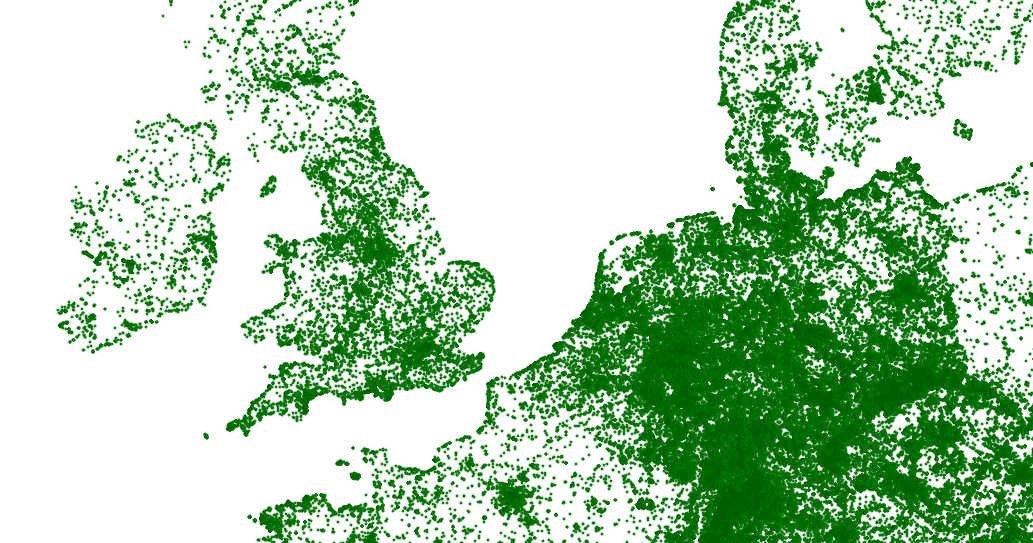
\includegraphics[scale=0.23]{figs/toomanyobjects.png}}
}

\frame
{
  \frametitle{Conflict sets}
  \emph{Different pieces of information have to '{fight}' for their representation in a specific level of detail - Monika Sester}
  
  \begin{center}
  	\fbox{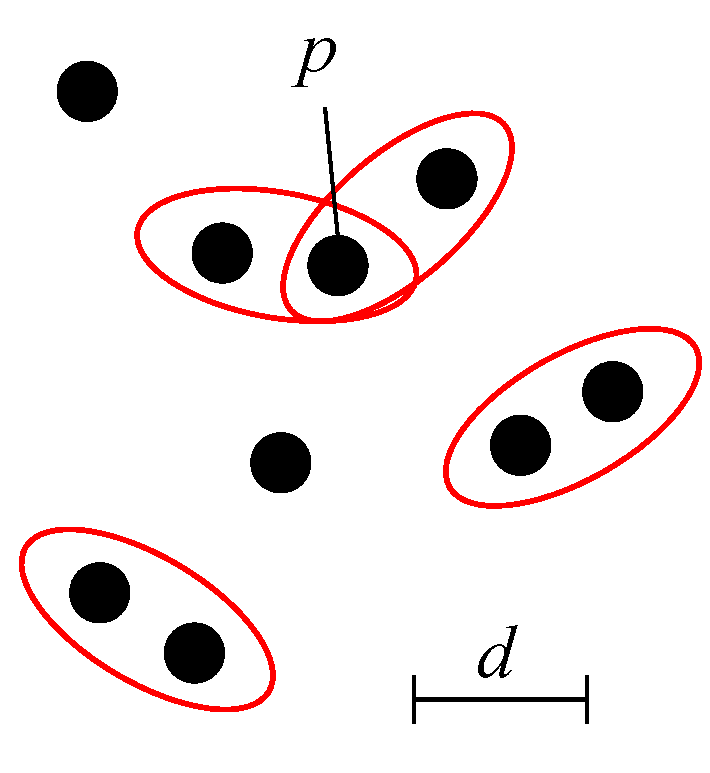
\includegraphics[scale=0.20]{figs/cvl_proximity_conflicts.pdf}} \fbox{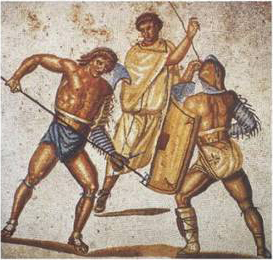
\includegraphics[scale=.38]{figs/gladiators.jpg}}
  \end{center}
  
  \begin{itemize}
  \item A conflict is subset of records, a subset of which have to be eliminated
  \end{itemize}
}

\frame
{
  \frametitle{Constraints in (our) zoomable maps}
  General constraint:
  \begin{itemize}
  \item \emph{Zoom-consistency}: A given record may only appear (not disappear) as you zoom in 
  \end{itemize}
  
  User-defined constraints:
  \begin{itemize}
  \item \emph{Visibility}: Within a unit area of the map, at most $K$ records may be visible
  \item \emph{Proximity}: Any two records must be separated by distance $d$
  \item ... (other user defined constraints that fit the model)
  \end{itemize}
  Our optimization model:
  \begin{itemize}
  \item User-defined (or \emph{user-level}) constraints generate a set of \emph{conflicts sets} on a given zoom-level
  \item A conflict set is a constraint in our optimization model
  \end{itemize}
}




\frame
{
  \frametitle{Tsunami of definitions}
  Definitions:
  \begin{itemize}
  \item $R$ is the collection of all records
  \item Each record $r \in R$ has weight $w_r$ (models importance)
  \item There are $\mathcal{Z}$ zoom-levels $\lbrace 1, \dots \mathcal{Z} \rbrace$
  \item $C$ is the collection of conflict sets for all zoom levels
  \item Each conflict set $c \in C$ is associated with a zoom-level $z_c$
  \item A conflict set $c \in C$ is a set of records $R_c \subseteq R$, where at least $\lambda_c \geq 1$ records must be filtered out at zoom level $z_c$  
  \end{itemize}
}


% OPTIMIZATION
\frame
{
  \frametitle{Problem 1: Multi-scale filtering problem}
  \begin{itemize}
  \item 0-1 decision variable $x_{rz}$ for each record $r \in R$ and each zoom level $z \in \lbrace 1, \dots, \mathcal{Z} \rbrace$
  \item $x_{rz}$ is 1 if record $r$ is filtered out at zoom level $z$, and 0 otherwise
  \end{itemize}
\begin{align}
  \label{eq:objective}
  \min ~\sum_{r \in R} \sum_{z=1}^\mathcal{Z} &w_r x_{rz} \\
  \label{eq:zoom-consistency}
  \mbox{s.t.}~~~~~~~x_{rz} &\geq x_{rz'}, ~~~~r \in R, ~~1 \leq z < z' \leq \mathcal{Z} \\
  \label{eq:general-constraints}
  \sum_{r \in R_c, ~z = z_c} x_{rz} &\geq \lambda_c, ~~~~~~ c \in C \\
  x_{rz} & \in \{0, 1\}, ~~ r \in R, ~~1 \leq z \leq \mathcal{Z}
\end{align}
  
}


% APPROACH
\frame
{
  \frametitle{Problem 2: Single-scale filtering problem}
  
  \begin{itemize}
  \item Problem 1 is too hard to solve in practice; conflict set can be huge -- in the order of thousands or millions
  \item Solve in a greedy fashion by solving the problem at the largest scale first (corresponding to zoom level $\mathcal{Z}$)
  \item Surviving records at zoom level $\mathcal{Z}$ is input to problem at zoom level $\mathcal{Z} -1$ etc.
  \item Zoom-consistency constraint is automatically fulfilled
  \item Multi-scale problem is broken down into $\mathcal{Z}$ single-scale problems
  \end{itemize}
}

% APPROACH
\frame
{
  \frametitle{Problem 2: Single-scale filtering problem (cont)}
  
  \begin{itemize}
  \item $\bar{R} \subseteq R$ is the set of records that have survived up to a given zoom-level
  \item $\bar{C}$ be the collection of active conflict sets at this zoom level
  \end{itemize}

  \begin{align}
  \label{eq:objective-single}
  \min ~\sum_{r \in \bar{R}} &w_r x_r \\
  \label{eq:general-constraints-single}
  \sum_{r \in \bar{R}_c} x_r &\geq \lambda_c, ~~~~ c \in \bar{C} \\
  x_r & \in \{0, 1\}, ~~ r \in \bar{R}, ~c \in \bar{C}
  \end{align}

  \begin{itemize}
  \item This is the \emph{set multicover problem} (Generalization of set cover)
  \item Each element/conflict set $c \in C$ needs to be covered $\lambda_c \geq 1$ times by the sets/records $r \in R$
  \item Each set/record can be chosen at most once.
  \end{itemize}

}

% ALGORITHMS
\frame
{
  \frametitle{Algorithms for set multicover problem}
  Exploit: Many heuristics and approximation algorithms exist for set cover (can be adapted for set multicover problem):
  \begin{itemize}
  \item \textbf{SGA}: Sort conflict sets by $w_r$, and delete the $\lambda_c$ lightest elements (optimal for disjoint conflict sets, i.e. points + visibility)
  \item \textbf{LPGA}: Solve LP-relaxation, round solutions using a special trick (see Vazirani)
  \item Several additional algorithms exist which we didn't try (future work)
  \end{itemize}
}


% LANGUAGE
\frame
{
  \frametitle{CVL: Cartographic Visualization Language}
  So that was the math. How did we implement it?
  \begin{itemize}
  \item Users write CVL:
  \end{itemize}
  \fbox{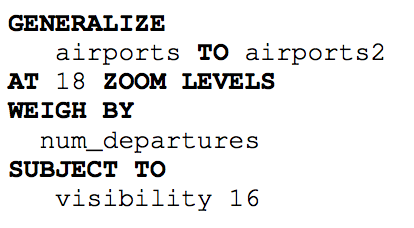
\includegraphics[scale=0.23]{figs/cvlexample.png}}
  
  \begin{itemize}
  \item CVL compiler generates a database program $P$ from CVL
  \item $P$ generates $\mathcal{Z}$ instances of problem 2 (one after the other)
  \item $P$ solves the instances (using database implementation of algorithm for set multicover problem)
  \item Algorithm to use is argument to CVL compiler
  \end{itemize}
}

% DEFINING CONSTRAINTS
\frame
{
  \frametitle{Defining constraints}
  Constraints are written in SQL: \\
  \fbox{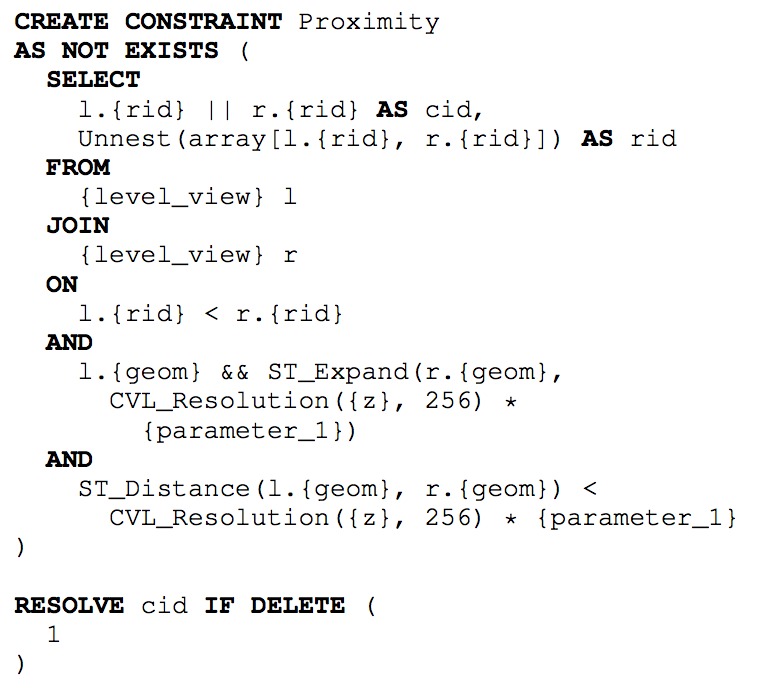
\includegraphics[scale=0.20]{figs/constraintexample.png}}\\
  \begin{itemize}
  \item 'AS NOT EXISTS' could be changed to 'GENERATE CONFLICTS AS'
  \end{itemize}
}

% RELATED WORK
\frame
{
  \frametitle{What does a result look like?}
  The result of running the example CVL script on a database of spatial data:\\
  \fbox{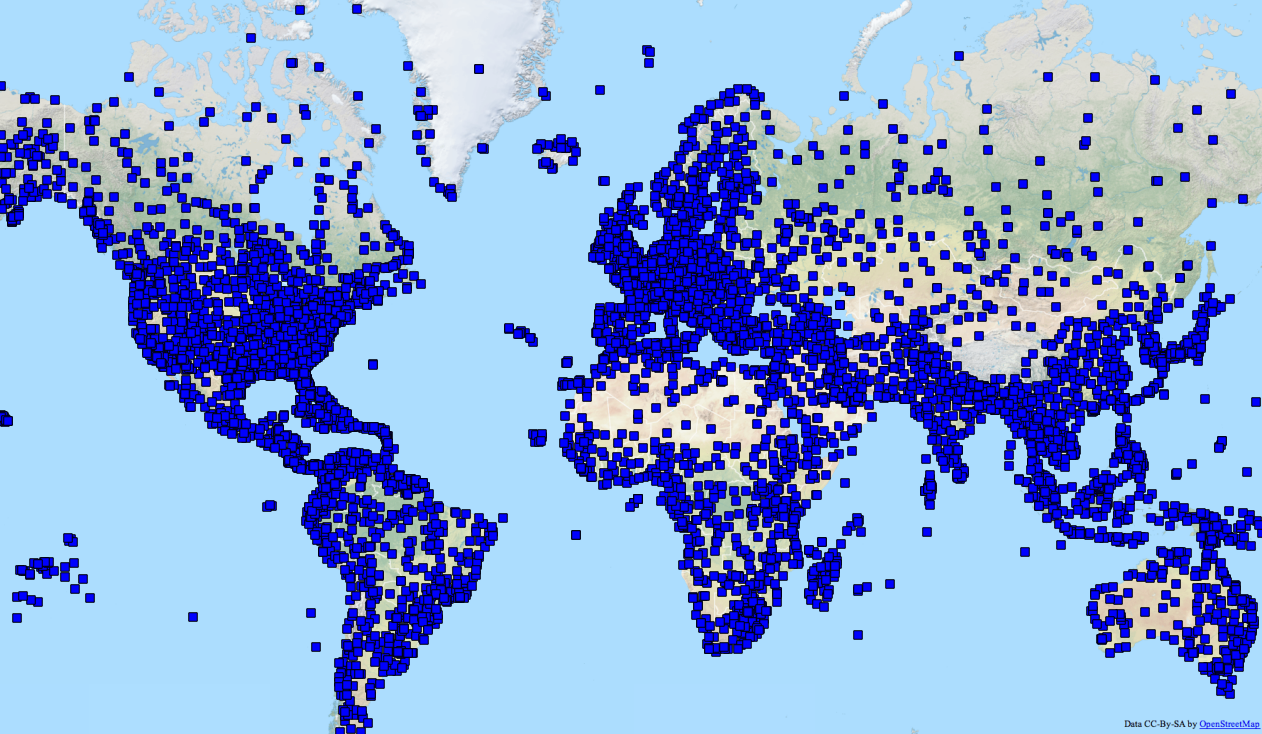
\includegraphics[scale=0.1]{figs/airports.png}}
  \fbox{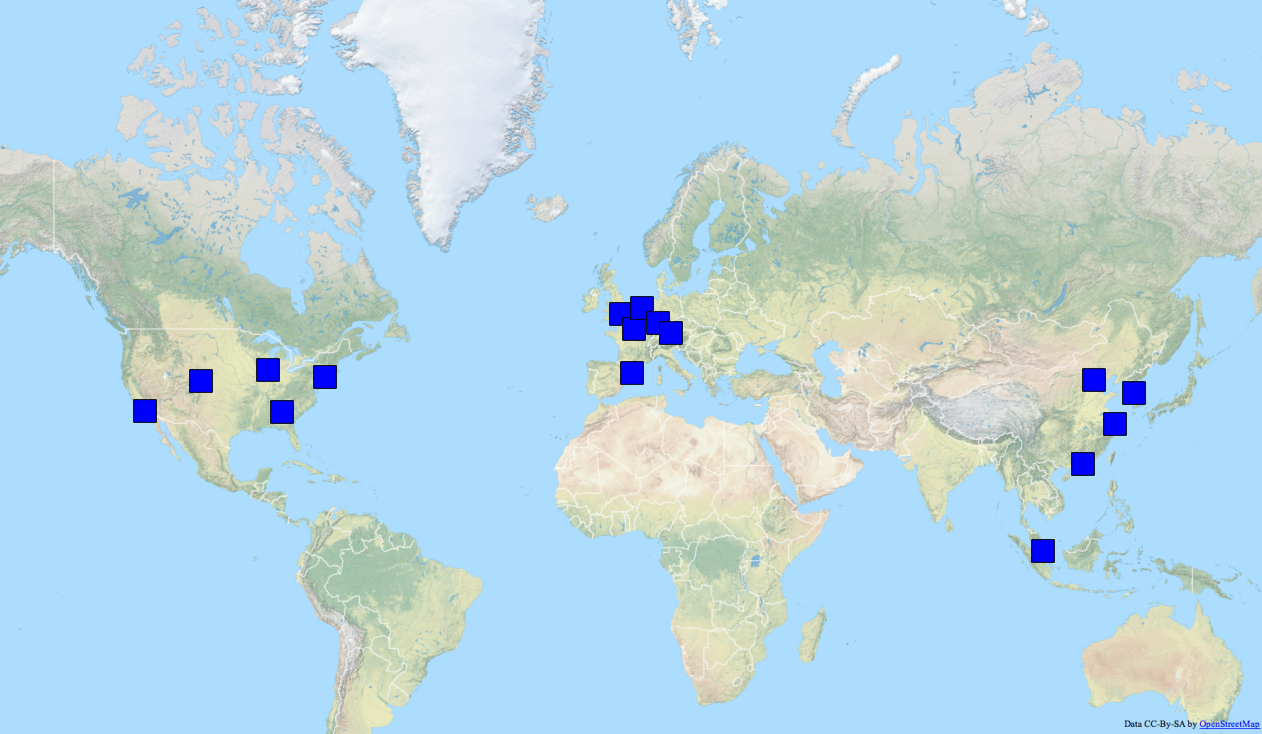
\includegraphics[scale=0.1]{figs/airports_z0.png}}
}


% RELATED WORK
\frame
{
  \frametitle{Related work}

  \begin{itemize}
  \item \emph{Reverse data management}, Meliou, A., Gatterbauer, W., \& Suciu, D. (2011).
  \item \emph{Efficient Spatial Sampling of Large Geographical Tables}. Das Sarma, A., Lee, H., Gonzalez, H., Madhavan, J., \& Halevy, A. (2012).
  \item \emph{Generalization of land cover maps by mixed integer programming}. Haunert, J.-H., \& Wolff, A. (2006). 
  \item \emph{Constant information density in zoomable interfaces}. Woodruff, A., Landay, J., Stonebraker, M. (1998).
  \end{itemize}
}

% Past and future work
\frame
{
  \frametitle{Past and future work}

  \begin{itemize}
  \item Past work: \emph{TileHeat}, predicting where people will look on a map tomorrow
  \item Latest work: \emph{Declarative Cartography}, the work described in these slides
  \item Future work: \emph{Real-time Declarative Cartography}, joint work with people at University of Zurich (Department of Geography)
  \item Future work: Succinct data representation of high-fidelity spatial data that is visualized on a digital map on a screen (think: pixel precision is not all that good)
  \end{itemize}
}




\end{document}
